\section{Readout Electronics}
\label{sec:dp-pds-electronics}

%%%%%%%%%%%%%%%%%%%%%%%%%%%%%%%%%
\subsection{Photomultiplier High Voltage Dividers}
\label{sec:fddp-pd-4.1}

The \dword{pmt} has a grounded cathode and a positive \dword{hv} applied to the anode. A single cable for each \dword{pmt} carries both power and signal. This configuration, which requires half as many cables and feedthroughs on the detector than the negative voltage configuration, offers a clear advantage given the large number of \dwords{pmt} in the detector. In addition, the cathode grounding shows fewer dark counts than the anode grounding scheme. Although a coupling capacitor must be used to separate the \dword{hv} from the \dword{pmt} signal, this signal and power splitting can be done externally, mitigating this drawback.  Figure~\ref{fig:dppd_4_1} shows the positive power supply and cathode grounding scheme.

\begin{dunefigure}[Positive power supply and cathode grounding scheme]{fig:dppd_4_1}
{Positive power supply and cathode grounding scheme.}
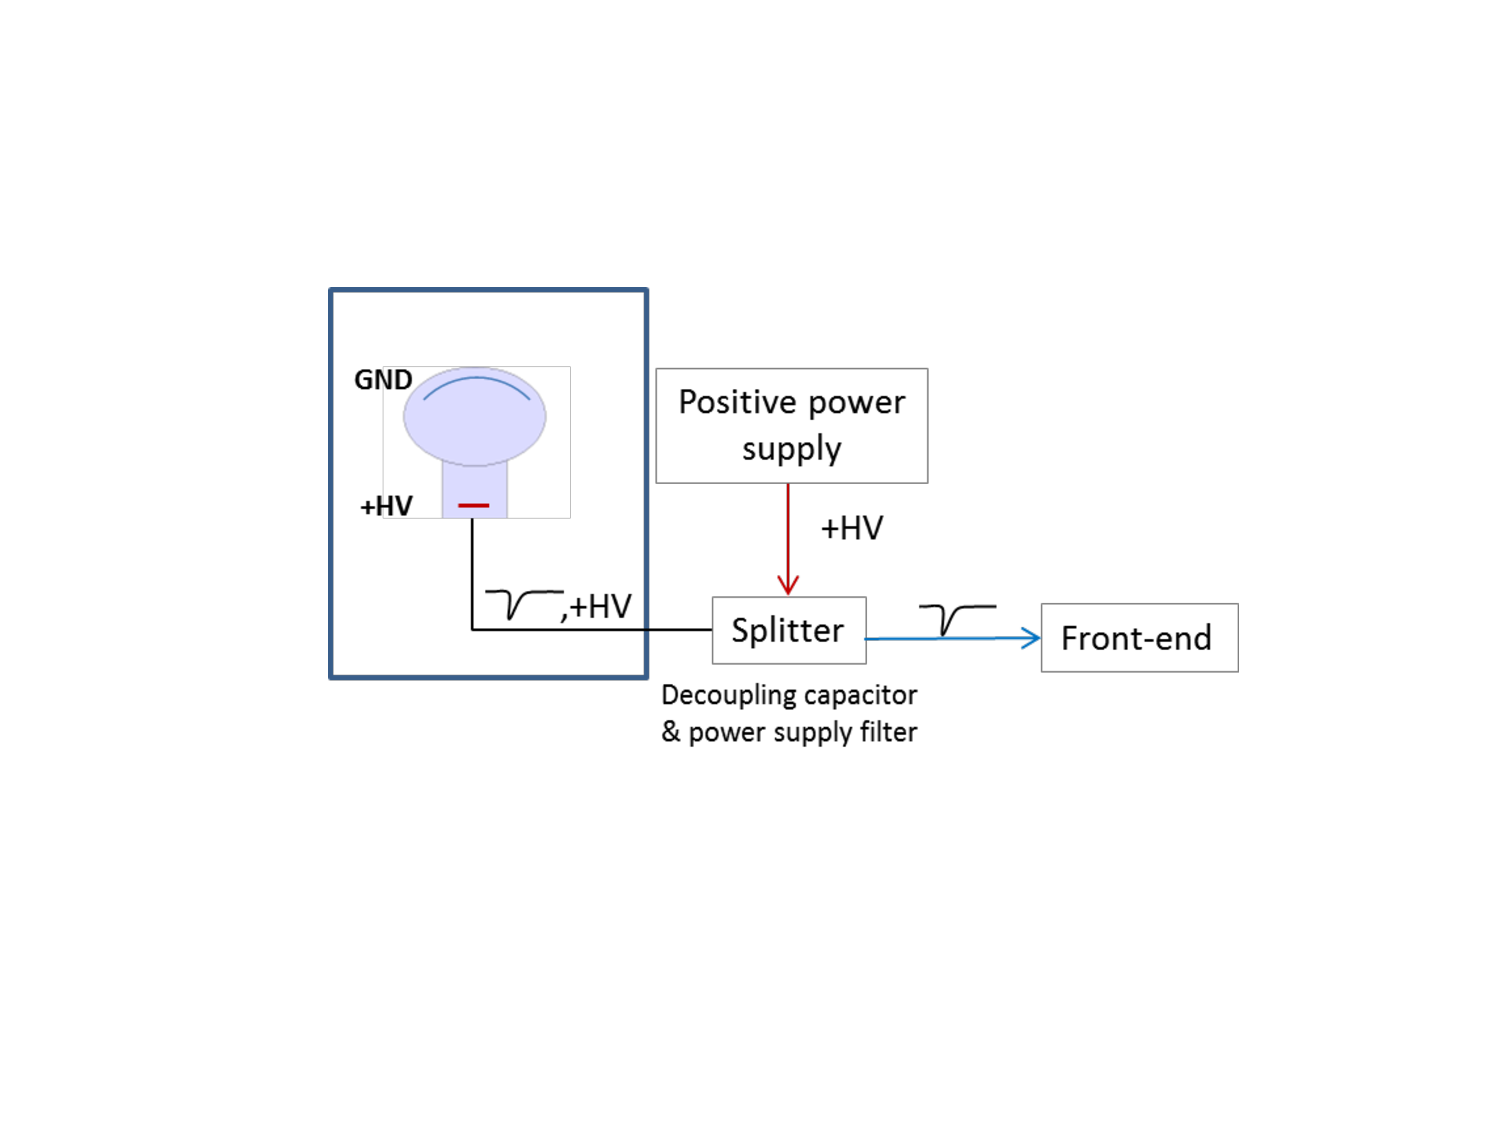
\includegraphics[width=0.6\textwidth]{dppd_4_1}
\end{dunefigure}

The \dword{pmt} base circuit uses only resistors and capacitors. The components are carefully selected and tested to minimize variations in their characteristics with temperature. The polarization current of the voltage divider (total circuit resistance) is chosen to fit the \dword{pmt} light linearity range (up to \SI{100}{PEs} per \SI{6}{\ns}, see Table~\ref{tab:specs:DP-PDS}) and maximum power requirements (\SI{<0.2}{W/\dword{pmt}}). The dynodes' voltage ratio will follow manufacturer recommendations for increasing linearity range on the space-charge effect area (tapered divider). In addition, capacitors are added to the last stages  to increase the \dword{pmt} linearity in pulsed mode.

The \dword{pmt} base connects to the \fdth with the RG-303/U cable, selected for its low attenuation and its proven reliability in cryogenic environments. The short cable is directly soldered to the \dword{pmt} base on one end and, on the other end, attaches to the long \dword{hv} cable with an SHV connector. The long cable connects to the feedthrough flange.

%This cable is directly soldered to the \dword{pmt} base on one side, and it ends with an SHV connector on the other side for attachment to the long \dword{hv} cables coming from the feedthrough flanges. 

%%%%%%%%%%%%%%%%%%%%%%%%%%%%%%%%%
\subsection{High Voltage and Signal Splitters}
\label{sec:fddp-pd-4.2}

\Dword{hv} and signal splitters 
separate the fast \dword{pmt} response signal from the positive \dword{hv} with capacitive decoupling. 
A low-pass filter between the \dword{hv} supply and the \dword{pmt} reduces the noise.

It is possible for radiated \dword{emi} picked up by the cables, and for conducted noise from the \dword{hv} power supply, to be synchronous across many \dword{pmt} channels (i.e., coherent noise). This noise could add up to produce false detector triggers. Because the \dword{pmt} signal can be as low as a few \si{mV},
control of the \dword{emi} over the circuit is very important. The splitter \dword{hv} input filter should reduce the \dword{emi} induced and conducted by the power supply cables. Enclosing each splitter channel in its own metallic grounded box reduces the \dword{emi} directly received in the splitter circuit and 
the cross-talk between different splitter channels.

Figure \ref{fig:dppd_4_2} shows a generic splitter circuit where R1 and C1 form the \dword{hv} input low-pass filter (with a cut-off frequency below \SI{60}{Hz}). The resistor R7 and the  \dword{led} are for safety only, warning when \dword{hv} is applied to the splitter. The C4 capacitor splits the signal coming from the \dword{pmt} from the \dword{hv}, and R2 prevents the \dword{pmt} signal from going to ground through the C1 capacitor. R4 and R5 are \SI{0}{\ohm} optional resistors that allow some flexibility in the grounding configuration. Finally, R3 ensures the discharging of C4 if the splitter is not connected to the \SI{50}{\ohm} input at the \dword{daq} system. The RC time constant of the capacitor C4 and the load (\SI{50}{\ohm}) must be as large as possible to minimize baseline oscillations due to the charge-discharge of the capacitor. Values of C4 between \SI{150}{nF} and \SI{300}{nF} have already been tested. Figure \ref{fig:dppd_4_3} shows the \dword{hv}/signal splitter box of \dword{pddp}.

\begin{dunefigure}[Generic splitter circuit diagram]{fig:dppd_4_2}
{Generic splitter circuit diagram.}
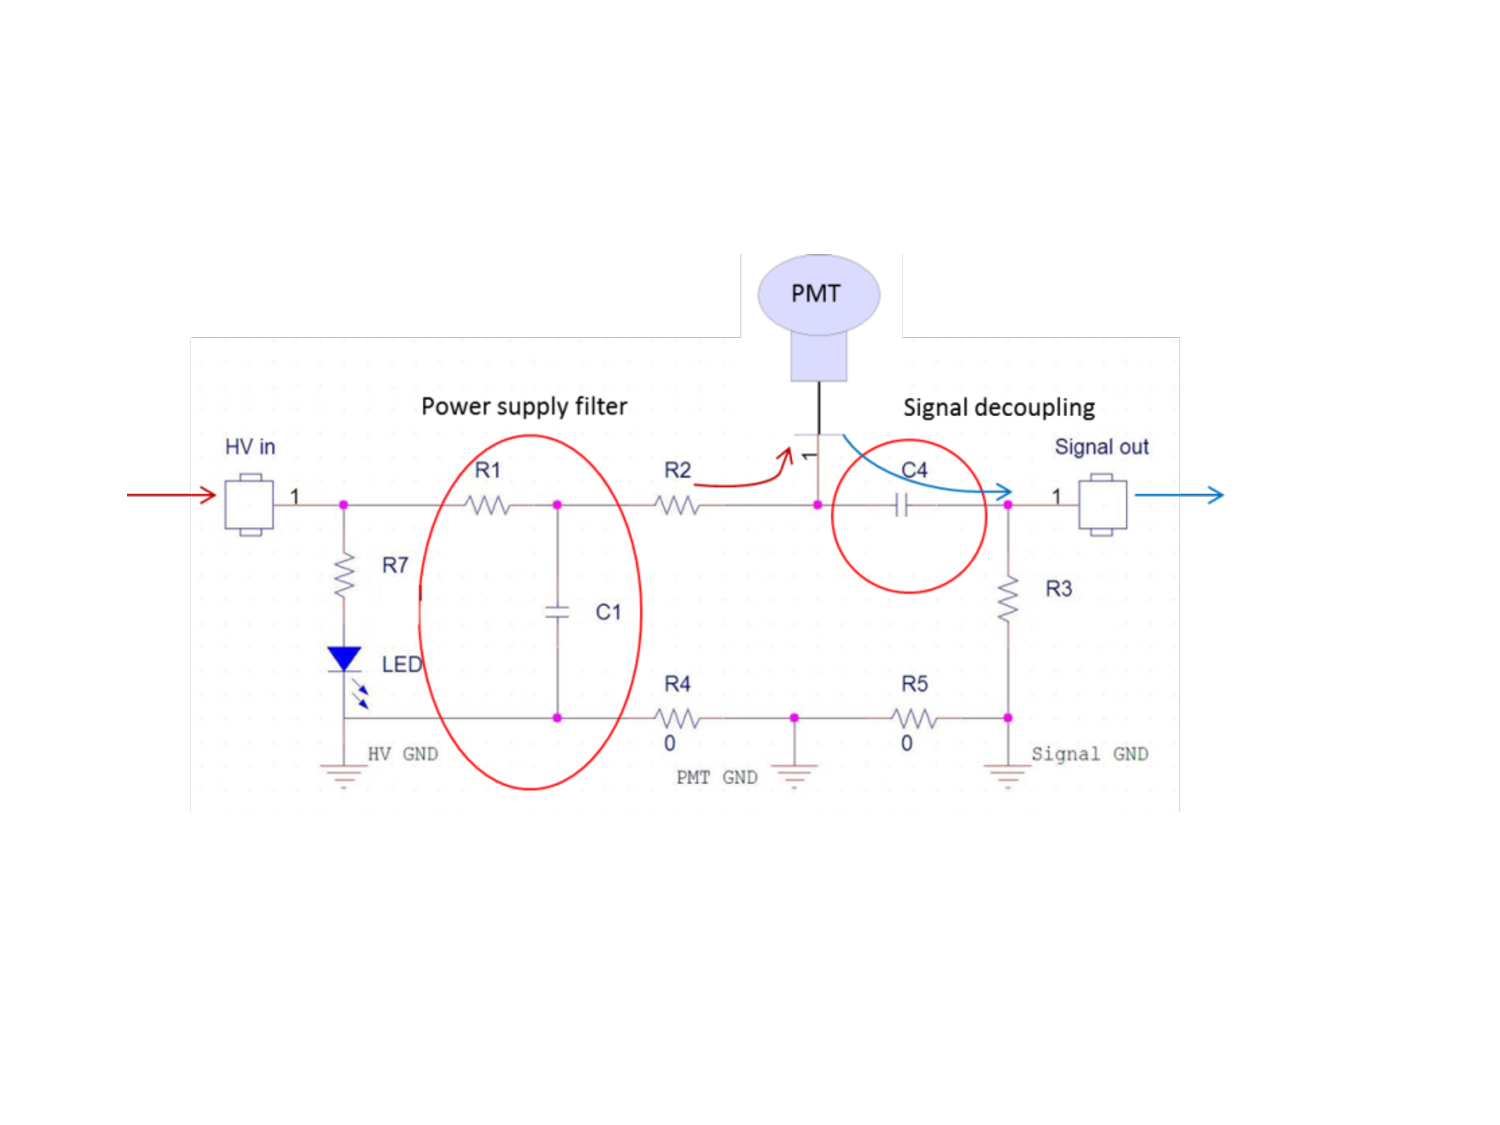
\includegraphics[width=0.85\textwidth]{dppd_4_2}
\end{dunefigure}

\begin{dunefigure}[Picture of the splitter box for \dshort{pddp}]{fig:dppd_4_3}
{Picture of the splitter box for \dword{pddp}.}
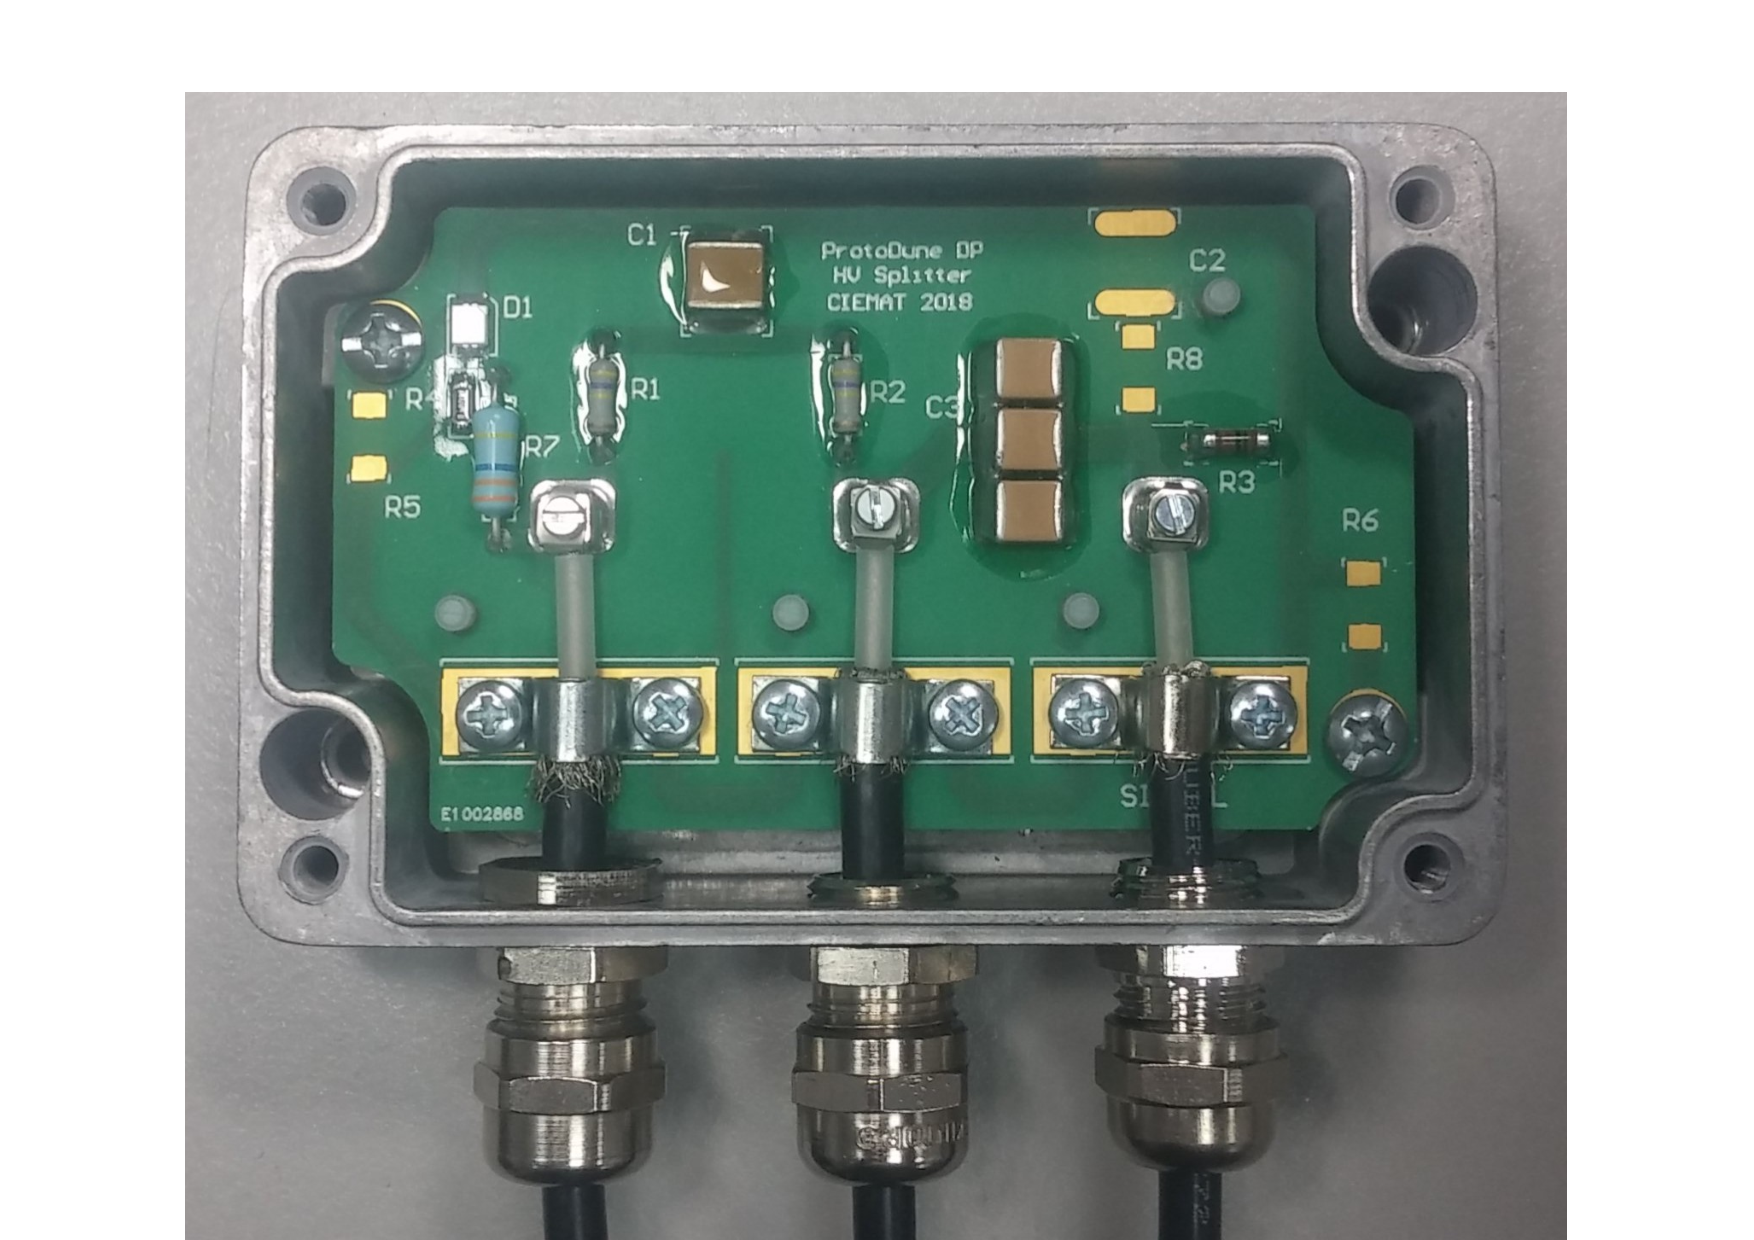
\includegraphics[width=0.5\textwidth]{dppd_4_n3}
\end{dunefigure}

For the connections between the \dword{hv} power supply and the splitters and between the splitters and the cryostat \fdth{}s, HTC 50-3-2 cables have been chosen as baseline. The HTC 50-3-2 has a similar attenuation as the RG-303/U (used inside the cryostat), but costs \numrange{8}{10} times less. Both cables are attached on one end directly to the \dword{hv} splitter and have an SHV connector on the other end. An RG-58 cable terminated on the connector required by the light readout card provides the connection between the splitter and the card. The \dword{pmt} readout card is described in Chapter~\ref{ch:dp-tpcelec}.

%\fixme{Add Antonio's picture of \dword{pddp} HV/signal splitter.}

%%%%%%%%%%%%%%%%%%%%%%%%%%%%%%%%%
%\subsection{Signal Readout Requirements}
\subsection{Signal Readout}
\label{sec:fddp-pd-4.3}

To meet the physics requirements, the following is the information that must be extracted from the \dword{pmt} signals:

\begin{itemize}
\item S1 fast component shape, charge, and timing;
\item S1 slow component shape and charge;
\item S2 shape, charge, and timing (distance from S1 and duration);
\item \dword{spe} charge spectrum for gain calculation during \dword{pmt} calibration;
\item trigger signal generation by the coincidence of several \dword{pmt} signals.
\end{itemize}

%%At this moment, we do not have an estimate of the \textbf{dynamic range }of the light that could reach the \dwords{pmt} on the \dword{dpmod}. Our calculations are based on the signals detected by the \dwords{pmt} on the  \dword{wa105} $3\times1\times1$\,m$^3$ detector. Although this prototype has a different dimension from the \dword{dpmod}, it is the only reference that we have for these estimates, until the \dword{pddp} detector and simulations are operational.
%There is currently no estimate on the dynamic range of the light expected to reach the \dwords{pmt} in the \dword{dpmod}. Our calculations are based on the signals detected by the \dwords{pmt} in the \dword{wa105}, % $3\times1\times1$\,m$^3$ detector. Although this prototype has a 
%which has quite different dimensions from the \dword{dpmod}. However, it is the only available reference %that we have for these estimates, until the \dword{pddp} and simulations are operational.

The requirements to both unambiguously reconstruct single-PE short pulses and to avoid saturation of S1 light signals of hundreds of PEs integrated charge distributed over hundreds of nanoseconds determine the readout electronics parameters, in particular \dword{pmt} gain readout sampling time. The \dword{pmt} gains will be set to \num{1e7} and the sampling time to \SI{15.4}{ns}, as justified in the following. In general, the \dword{pmt} signal dynamic range goes from the \si{mV} level to several volts (over \SI{50}{\ohm} load). The lower limit of the \dword{pmt} dynamic range is given by the lowest level of the \dword{spe} signal that meets the signal to noise ratio specification. Thus, the \dword{pmt} gain should be set at least at the value that makes the \dword{spe} level meet this condition. Figure~\ref{fig:dppd_4_3_ab} shows the \dword{spe} waveforms (left) and amplitudes from the WA105 at different voltages (right).

\begin{dunefigure}[\dshort{spe} waveforms and amplitudes from the WA105 at different voltages]{fig:dppd_4_3_ab}{\dword{spe} waveforms (left) and amplitudes from the WA105 at different voltages (right).}
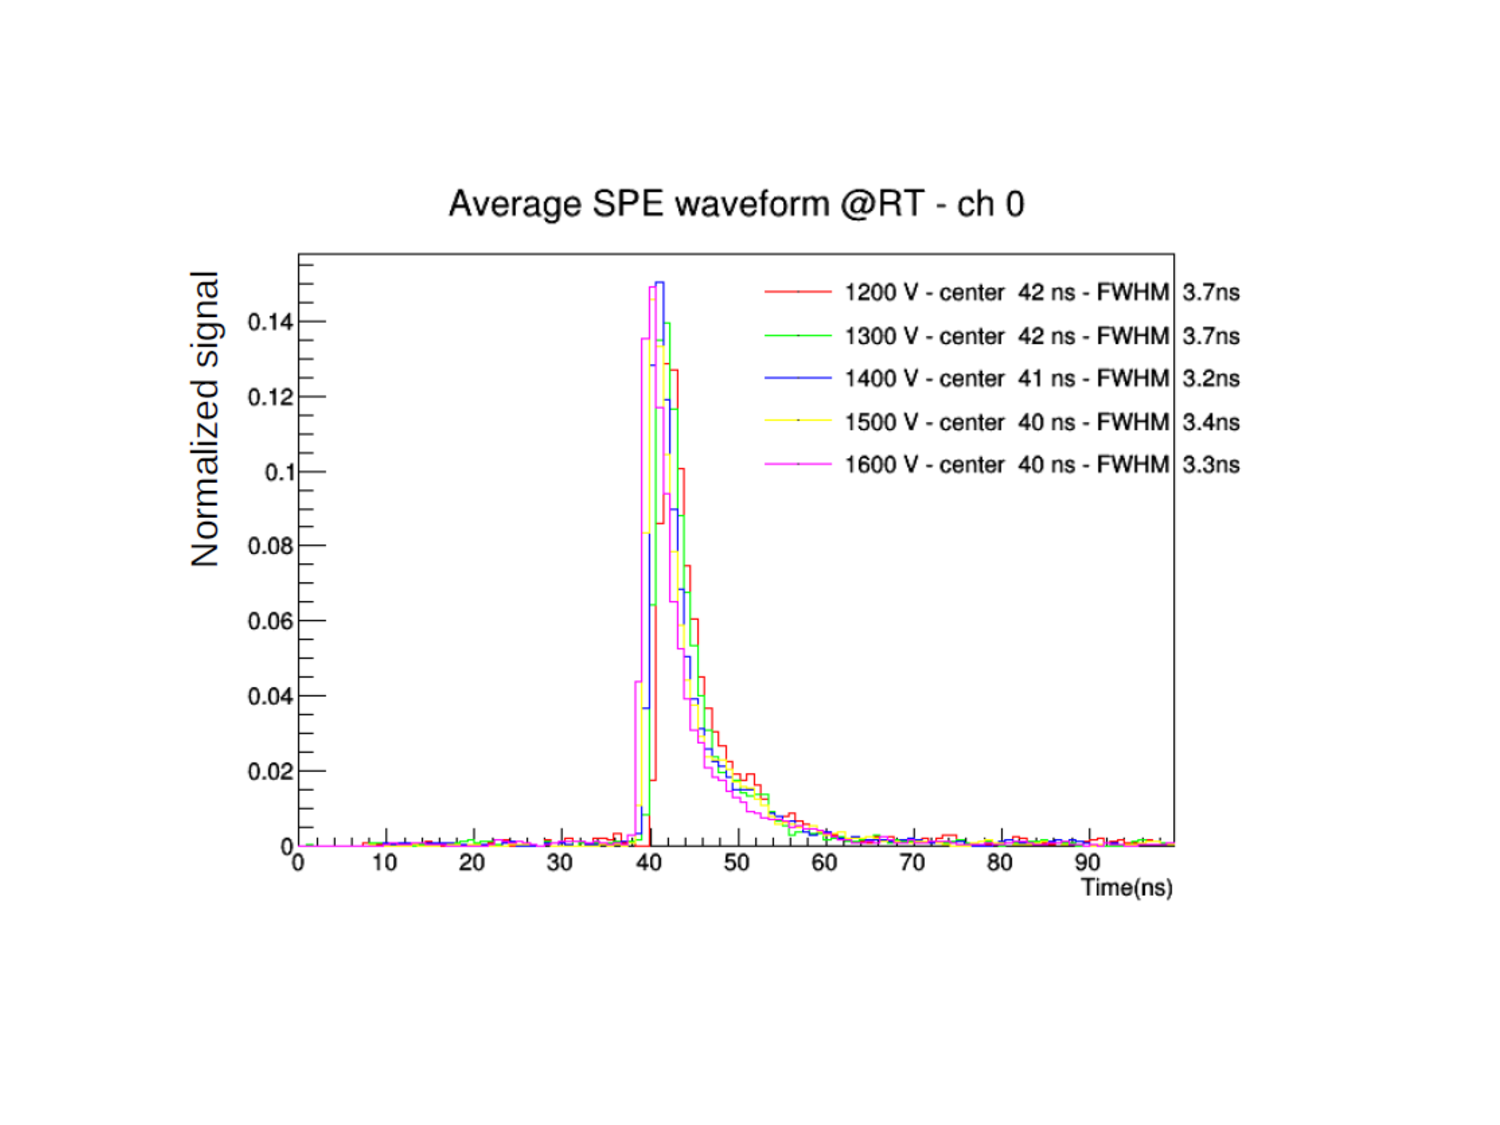
\includegraphics[width=0.47\textwidth]{dppd_4_3_a}
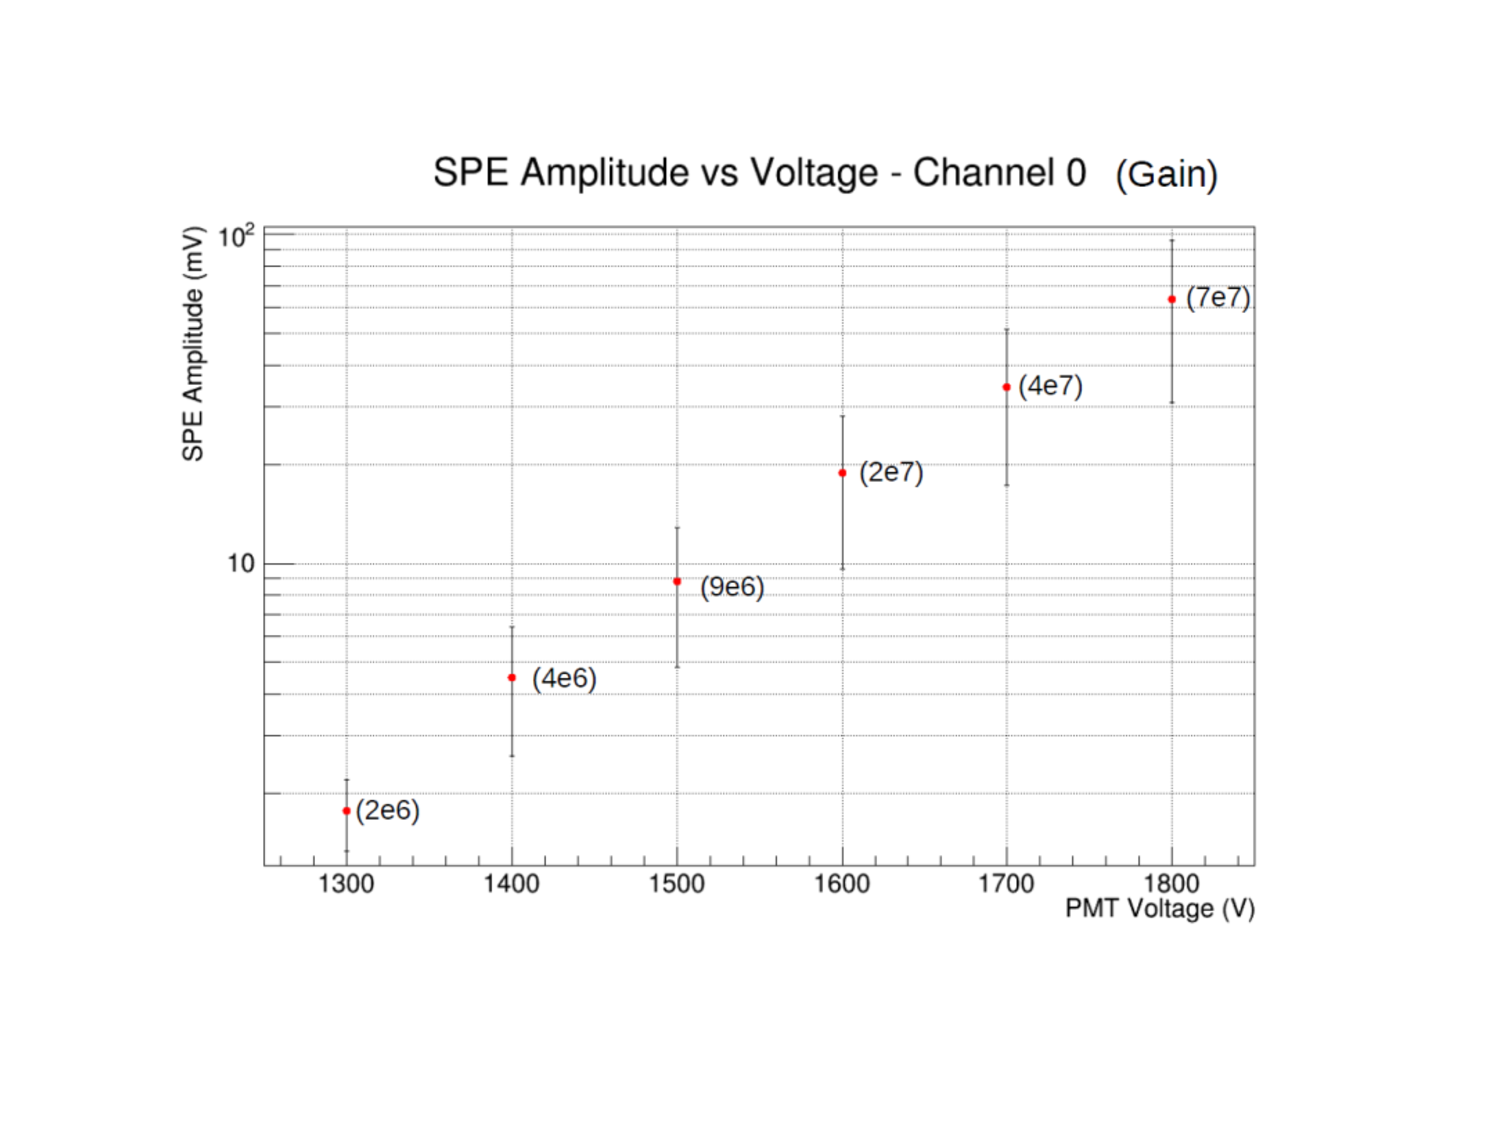
\includegraphics[width=0.47\textwidth]{dppd_4_3_b}
\end{dunefigure}

Because the long cables from the \dwords{pmt} to the \dword{fe} electronics are very long, the cable noise could be high. If a noise level around \SI{1}{mV} is considered,  the \dword{pmt} gain must be set to \num{e7} or higher to have the required S/N ratio of 5, see Table~\ref{tab:specs:DP-PDS}. The average \dword{spe} pulse width is approximately \SI{3.5}{ns} \dword{fwhm}. If an accurate signal reconstruction is required, the sampling period should be of the level of the \si{\ns}. Since only charge information and approximate timing information (at the level of $<\,\SI{100}{ns}$ RMS hit time resolution, see Table~\ref{tab:specs:DP-PDS}) is necessary, the sampling period can be higher, but the signal must be low-pass filtered before sampling. This filtering affects the signal level making the discrimination of signal from noise more difficult, requiring an increase of the \dword{pmt} gain to meet the S/N specification. 

%The sampling frequency also affects the time tagging precision. The time uncertainty due to the \dword{pmt} alone is approximately \SI{3}{ns} (transit time spread). Other factors, like Rayleigh scattering, increase this uncertainty, as does the sampling period. 

The upper limit of the required dynamic range is given by the \dword{pmt} signal amplitude for the maximum number of \dwords{pe} expected per sampling time unit. As shown in Figure~\ref{fig:dppd_saturation} for simulated \SI{3}{GeV} beam neutrino interactions, the maximum number expected in this case is about \SI{60}{PEs} for a fast sampling of \SI{4}{ns} and about \SI{500}{PEs} for sampling times comparable to S1 signal durations (about \SI{1}{\micro\second}) or slower. Hence, while single-PE signals can  still be detected with slow sampling times by adjusting the \dword{pmt} gain accordingly, the dynamic range requirement becomes more stringent. 

The time sampling of the \dword{pds} waveforms will be \SI{15.4}{ns}, as provided by the \SI{65}{MHz} ADC in the \dword{lro} electronics card (see Section~\ref{ch:dp-tpcelec}). Similar readout electronics parameters as the baseline ones described here are being validated in \dword{pddp}, and are found to meet our specifications. In particular, Hamamatsu R5912-MOD20 \dwords{pmt} operated at a gain of \num{1e7} and whose signals are digitized at a \SI{16}{ns} sampling period yield a single-\dword{pe} signal-to-noise ratio in excess of the required S/N=5 value.

%Therefore, the higher the sampling frequency, the better for detector performance but at the cost of increased data rate and storage requirements.


The light signal must be synchronized with the \dword{daq}. All \dword{daq} electronics use the \dword{wr} protocol for synchronization. A dedicated \dword{wr} \dword{utca}~\cite{utca} slave node is on the light readout \dword{fe} electronics as sync receiver, distributing clocks to different \dword{fe} cards.

